
\begin{enumerate}
\item A ball is thrown from ground at an angle $\theta$ with horizontal and with an initial speed $u_0$. For the resulting projectile motion, the magnitude of average velocity of the ball up to the point when it hits the ground for the first time is $V_1$. After hitting the ground, the ball rebounds at the same angle $\theta$ but with a reduced speed of $u_0/\alpha$. Its motion continues for a long time as shown in figure. If the magnitude of average velocity of the ball for entire duration of motion is $0.8 V_1$, the value of $\alpha$ is \_\_\_\_\_\_\_.

\begin{center}
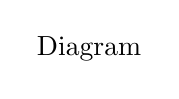
\begin{tikzpicture}
\node {Diagram};
\end{tikzpicture}
\end{center}

\end{enumerate}
